%%%%%%%%%%%%%%%%%%%%%%%%%%%%%%%%%%%%%%%%%%%%%%%%%%%%%%%%%%%%%%%%%%%%%%%%%%%%%%%
%                       CARREGA DE LA CLASSE DE DOCUMENT                      %
%                                                                             %
% Les opcions admissibles son:                                                %
%      12pt / 11pt            (cos dels tipus de lletra; no feu servir 10pt)  %
%                                                                             %
% catalan/spanish/english     (llengua principal del treball)                 %
%                                                                             % 
% french/italian/german...    (si necessiteu fer servir alguna altra llengua) %
%                                                                             %
% listoffigures               (El document inclou un Index de figures)        %
% listoftables                (El document inclou un Index de taules)         %
% listofquadres               (El document inclou un Index de quadres)        %
% listofalgorithms            (El document inclou un Index d'algorismes)      %
%                                                                             %
%%%%%%%%%%%%%%%%%%%%%%%%%%%%%%%%%%%%%%%%%%%%%%%%%%%%%%%%%%%%%%%%%%%%%%%%%%%%%%%

\documentclass[11pt,spanish,listoffigures,listoftables]{tfgetsinf}

%%%%%%%%%%%%%%%%%%%%%%%%%%%%%%%%%%%%%%%%%%%%%%%%%%%%%%%%%%%%%%%%%%%%%%%%%%%%%%%
%                     CODIFICACIO DEL FITXER FONT                             %
%                                                                             %
%    windows fa servir normalment 'ansinew'                                   %
%    amb linux es possible que siga 'latin1' o 'latin9'                       %
%    Pero el mes recomanable es fer servir utf8 (unicode 8)                   %
%                                          (si el vostre editor ho permet)    % 
%%%%%%%%%%%%%%%%%%%%%%%%%%%%%%%%%%%%%%%%%%%%%%%%%%%%%%%%%%%%%%%%%%%%%%%%%%%%%%%

\usepackage[utf8]{inputenc} 

%%%%%%%%%%%%%%%%%%%%%%%%%%%%%%%%%%%%%%%%%%%%%%%%%%%%%%%%%%%%%%%%%%%%%%%%%%%%%%%
%                        ALTRES PAQUETS I DEFINICIONS                         %
%                                                                             %
% Carregueu aci els paquets que necessiteu i declareu les comandes i entorns  %
%                                          (aquesta seccio pot ser buida)     %
%%%%%%%%%%%%%%%%%%%%%%%%%%%%%%%%%%%%%%%%%%%%%%%%%%%%%%%%%%%%%%%%%%%%%%%%%%%%%%%
\usepackage{float}
\usepackage{glossaries}
\glstoctrue
\makeglossaries

\newglossaryentry{bug}
{
  name=Bug,
  description={Problema en un programa de computador o sistema de software que desencadena un resultado indeseado}
}

\newglossaryentry{JSON}
{
  name=\textit{JSON},
  description={ Acrónimo de \textit{JavaScript Object Notation}, es un formato de texto ligero para el intercambio de datos. Más información en \url{https://es.wikipedia.org/wiki/JSON}}
}

\newglossaryentry{python}
{
  name=Python,
  description={ Lenguaje de programación interpretado cuya filosofía hace hincapié en una sintaxis que favorezca un código legible.}
}

\setglossarystyle{altlisthypergroup}

%%%%%%%%%%%%%%%%%%%%%%%%%%%%%%%%%%%%%%%%%%%%%%%%%%%%%%%%%%%%%%%%%%%%%%%%%%%%%%%
%                        DADES DEL TREBALL                                    %
%                                                                             %
% titol, alumne, tutor i curs academic                                        %
%%%%%%%%%%%%%%%%%%%%%%%%%%%%%%%%%%%%%%%%%%%%%%%%%%%%%%%%%%%%%%%%%%%%%%%%%%%%%%%

\title{Un entorno colaborativo para el diseño, desarrollo y compilación de notebooks de trabajo Jupyter compartidos. }
\author{Javier Rodríguez Domínguez}
\tutor{José Manuel Bernabeu Aubán}
\curs{2017-2018}

%%%%%%%%%%%%%%%%%%%%%%%%%%%%%%%%%%%%%%%%%%%%%%%%%%%%%%%%%%%%%%%%%%%%%%%%%%%%%%%
%                     PARAULES CLAU/PALABRAS CLAVE/KEY WORDS                  %
%                                                                             %
% Independentment de la llengua del treball, s'hi han d'incloure              %
% les paraules clau i el resum en els tres idiomes                            %
%%%%%%%%%%%%%%%%%%%%%%%%%%%%%%%%%%%%%%%%%%%%%%%%%%%%%%%%%%%%%%%%%%%%%%%%%%%%%%%

\keywords{????, ?????????, ????, ?????????????????} % Paraules clau 
         {?????, ???, ???????????????}              % Palabras clave
         {?????, ????? ?????, ?????????????}        % Key words

%%%%%%%%%%%%%%%%%%%%%%%%%%%%%%%%%%%%%%%%%%%%%%%%%%%%%%%%%%%%%%%%%%%%%%%%%%%%%%%
%                              INICI DEL DOCUMENT                             %
%%%%%%%%%%%%%%%%%%%%%%%%%%%%%%%%%%%%%%%%%%%%%%%%%%%%%%%%%%%%%%%%%%%%%%%%%%%%%%%

\begin{document}

%%%%%%%%%%%%%%%%%%%%%%%%%%%%%%%%%%%%%%%%%%%%%%%%%%%%%%%%%%%%%%%%%%%%%%%%%%%%%%%
%              RESUMS DEL TFG EN VALENCIA, CASTELLA I ANGLES                  %
%%%%%%%%%%%%%%%%%%%%%%%%%%%%%%%%%%%%%%%%%%%%%%%%%%%%%%%%%%%%%%%%%%%%%%%%%%%%%%%

\begin{abstract}
????
\end{abstract}
\begin{abstract}[spanish]
????
\end{abstract}
\begin{abstract}[english]
????
\end{abstract}

%%%%%%%%%%%%%%%%%%%%%%%%%%%%%%%%%%%%%%%%%%%%%%%%%%%%%%%%%%%%%%%%%%%%%%%%%%%%%%%
%                              CONTINGUT DEL TREBALL                          %
%%%%%%%%%%%%%%%%%%%%%%%%%%%%%%%%%%%%%%%%%%%%%%%%%%%%%%%%%%%%%%%%%%%%%%%%%%%%%%%

\mainmatter



%%%%%%%%%%%%%%%%%%%%%%%%%%%%%%%%%%%%%%%%%%%%%%%%%%%%%%%%%%%%%%%%%%%%%%%%%%%%%%%
%                                  INTRODUCCIO                                %
%%%%%%%%%%%%%%%%%%%%%%%%%%%%%%%%%%%%%%%%%%%%%%%%%%%%%%%%%%%%%%%%%%%%%%%%%%%%%%%


\chapter{Introducci\'on}
\label{ch:intro}

Las herramientas para el trabajo colaborativo son un recurso muy utilizado a día de hoy. Se trate de editar un documento de texto por dos o más partes o de desarrollar una aplicación informática, existen plataformas para lograrlo de una manera muy sencilla, como podrían ser en estos casos \textit{Google Docs} \footnote{https://www.google.es/intl/es/docs/about/} \textit{Github} \footnote{https://github.com/}. 

Sin embargo, existen otras muchas plataformas que no disponen de la posibilidad de hacer un uso grupal de ellas. \textit{Jupyter} \footnote{http://jupyter.org/} pertenece a este último grupo, pues no ofrece una manera de editar sus \textit{notebooks} (los documentos con los que se trabaja) en tiempo real por más de un usuario a la vez. Para aquellos que no conozcan la plataforma, se va a realizar una introducción:

\textit{Jupyter } es una herramienta para la programación interactiva en diferentes leguajes. Nace como la sucesión natural de \textit{IPython} \textit{(Interactive Python)}. Se trata de un programa que extendía las funcionalidades de la propia terminal de \textit{\gls{python}} con la intención de que su uso fuera más interactivo. Más adelante, este proyecto pasaría a utilizar un sistema de \textit{notebooks}, como el que utilizan programas tan conocidos como \textit{Mathematica} \footnote{https://www.wolfram.com/mathematica/}. La estructura del \textit{notebook} es bastante sencilla. Internamente, el \textit{notebook} es un documento \textit{\gls{JSON}}, con bloques denominados celdas, los cuales tienen una entrada \textit{(input)} y una salida \textit{(output)}. Para que el \textit{notebook} sea legible, se visualiza de una manera ordenada, mostrando solo el código y los resultados obtenidos al usuario y haciendo que el uso de la herramienta sea lo más fluido posible.   
Esta mejora sería bastante significativa, pues se podía mantener una persistencia entre sesiones, ya que los \textit{notebooks} pueden ser guardados y cargados. El siguiente paso fué saltar al proyecto \textit{Jupyter}, cuyo cambio más importante fué la posibilidad de trabajar con lenguajes diferentes a \textit{python}. Ésto se consigue desacoplando la lógica de la ejecución del código del servicio principal de edición de \textit{notebooks}. El código a ejecutar se manda a un proceso que lo recibe, lo ejecuta y lo devuelve. Estos procesos se llaman \textit{Kernels}, y a día de hoy existen \textit{Kernels} para más de 100 lenguajes que pueden ser utilizados con \textit{Jupyter}.

Al no facilitar de manera nativa la colaboración entre usuarios, \textit{Jupyter} nos deja la posibilidad de trabajar mandando el \textit{notebook} entre los diferentes autores a medida que se va modificando. Ésto es un método poco eficiente, principalmente por dos razones. En primer lugar, \textit{Jupyter} tiene una mala interacción con los servicios de control de versiones, pues el usuario modifica las celdas, pero realmente lo que cambia es el \textit{JSON} interno. La herramienta de control de versiones busca los cambios entre estos documentos \textit{JSON}, y encuentra muchas más diferencias de las que se realizaron por los usuarios, pues ellos solo alteraron las celdas, pero internamente estos cambios se representaron de una forma mucho más extensa.
Por otro lado, \textit{Jupyter} es ampliamente utilizado en entornos de análisis de datos. En estas circunstancias, se suele trabajar con grandes cantidades de información, que tiene que ser cargada y procesada. Cuando se comparte un notebook, se comparte sólo el \textit{JSON} que lo forma, no el estado de ejecución del \textit{Kernel}. Esto quiere decir que cada vez que alguien quiere hacer una prueba con los datos, tiene que procesarlos y cargarlos en memoria, computaciones que pueden ser bastante costosas.

En resumen, trabajar de forma colaborativa haciendo uso de \textit{Jupyter} a día de hoy es una tarea complicada debido a la naturaleza de la plataforma, y, al ser muy utilizada en este tipo de situaciones, nos plantea un problema que puede ser de gran ayuda resolver.


% MOTIVACIÓN

\section{Motivaci\'on}
\label{sec:motivacion}

A la hora de plantear el tema para el Trabajo de Fin de Grado, se propusieron dos temas principalmente. El primero fué la adaptación de la base de datos \textit{RethinkDB} \footnote{https://www.rethinkdb.com/} para introducirla como un componente en un sistema de \textit{PaaS}. Por otro lado se planteó la creación de un entorno colaborativo para el diseño, desarrollo y compilación de notebooks de trabajo \textit{Jupyter} compartidos. Después de estudiar las dos opciones a fondo, me decanté por la segunda propuesta, pues ya había hecho uso de la plataforma y me había enfrentado a los problemas que supone utilizarla en un ámbito colaborativo.

\textit{Jupyter} es una plataforma que puede ser utilizada para diversos fines, ya que la manera que tiene de presentar el código y los resultados es muy visual. Ésto ha hecho que sea un recurso muy utilizado en entornos donde es importante entender qué hace cada trozo de código, como por ejemplo en la educación o en el análisis de datos. En estas situaciones se trabaja mucho en grupos, y la posibilidad de utilizar \textit{Jupyter} de manera colaborativa entre los miembros de estos grupos puede facilitar mucho el desarrollo de los proyectos.

Existen herramientas que proponen un \textit{Jupyter} colaborativo a través de internet, como \textit{Google Colab} \footnote{https://colab.research.google.com} o \textit{CoCalc} \footnote{https://cocalc.com/}. Estas plataformas permiten una edición de los \textit{notebooks} simultánea, haciendo que dos o más usuarios puedan modificar los contenidos del \textit{notebook} a la vez y sin control alguno. Desde mi punto de vista, este enfoque a un \textit{Jupyter} colaborativo no es el más adecuado, y pienso que un entorno con políticas más restrictivas en cuanto a la modificación de los documentos puede ser más acorde con el modelo de ejecución.

A nivel personal, pienso que tomar como base para mi Trabajo de Fin de Grado un proyecto real puede ser muy beneficioso, ya que tengo la oportunidad de ver como se trabaja en entornos profesonales. Además, me tengo que enfrentar a problemas nuevos para mí, como el diseño de una arquitectura o la implementación de un servicio web. 


% OBJETIVOS

\section{Objetivos}
\label{sec:objetivos}

El objetivo principal del proyecto es el desarrollo de un entorno colaborativo para \textit{Jupyter}. Entendemos desarrollo como todo el proceso creativo, desde la concepción de la idea y el diseño formal hasta la implementación final del código.

En cuanto a objetivos más acotados y específicos, tenemos los siguientes, cada uno con su correspondientes apartados de diseño e implementación:
\begin{itemize}
\item Sincronizar los \textit{notebooks} en tiempo real.
\item Crear un sistema de roles y permisos para los usuarios.
\item Autenticar a los usuarios.
\item Compartir los documentos.
\item Persistir la información necesaria.
\item Mantener las sesiones de los usuarios.
\end{itemize}

Estos objetivos específicos se pueden entender como pequeños apartados que, una vez unidos y cohesionados, supondrán el cumplimiento del objetivo principal.


% IMPACTO ESPERADO

\section{Impacto esperado}
\label{sec:impacto}

Se espera que la herramienta resultante facilite el uso de \textit{Jupyter} en situaciones colaborativas, reduciendo el tiempo y esfuerzo empleado en poner en común los cambios que se vayan a realizar. También se pretende que se trabaje en tiempo real, agilizando todo el proceso de desarrollar la tarea en cuestión. 


% METODOLOGÍA

\section{Metodología}
\label{sec:metodologia}

La metodología seguida para el desarrollo del trabajo ha sido la siguiente. Siguiendo los objetivos marcados, se ha procedido a realizar primero un diseño estructural de cada una de las partes. Este diseño se ha comparado con otros exhaustivamente para elegir el que mejor se adecuara al apartado tratado. Más tarde se procede a implementar la parte en base al diseño, y por último a hacer pruebas con el fin de encontrar fallos o \textit{\gls{bug}s} y poder solucionarlos.


% ESTRUCTURA DE LA MEMORIA

\section{Estructura de la memoria}
\label{sec:estructura}

La memoria seguirá una estructura bastante convencional según la guías que ofrece la UPV. Comenzaré hablando del estado del arte en el capítulo \ref{ch:state-of-art}, donde haré una comparativa de \textit{Jupyter} con plataformas similares, en los capítulos \ref{ch:analisis-problema}, \ref{ch:diseno-solu} y \ref{ch:desarrollo-solucion} se planteará el problema, las diferentes soluciones propuestas para resolverlo, así como el diseño y desarrollo de éstas. En los dos capítulos siguientes, \ref{ch:implantacion} y \ref{ch:pruebas} hablaré de la implantación del sistema, cómo desplegarlo y ponerlo en marcha, así como de las pruebas realizadas a éste. Por último, se hará una conclusión del trabajo, exponiendo si se han alcanzado los objetivos y de que manera, y se propondrán mejoras que se pueden llevar a cabo en un futuro, capítulos \ref{ch:conclusiones} y \ref{ch:futuro}. 

%\section{Notes bibliografiques} %%%%% Opcional

%????? ????????????? ????????????? ????????????? ????????????? ?????????????

%%%%%%%%%%%%%%%%%%%%%%%%%%%%%%%%%%%%%%%%%%%%%%%%%%%%%%%%%%%%%%%%%%%%%%%%%%%%%%%
%                         CAPITOLS (tants com calga)                          %
%%%%%%%%%%%%%%%%%%%%%%%%%%%%%%%%%%%%%%%%%%%%%%%%%%%%%%%%%%%%%%%%%%%%%%%%%%%%%%%



%%%%%%%%%%%%%%%%%%%%%%%%%%%%%%%%%%%%%%%%%%%%%%%%%%%%%%%%%%%%%%%%%%%%%%%%%%%%%%%
%                                 ESTADO DEL ARTE                             %
%%%%%%%%%%%%%%%%%%%%%%%%%%%%%%%%%%%%%%%%%%%%%%%%%%%%%%%%%%%%%%%%%%%%%%%%%%%%%%%


\chapter{Estado del arte}
\label{ch:state-of-art}


\section{Crítica al estado del arte}
\label{sec:critica-estado}

\section{Propuesta}
\label{sec:propuesta}



%%%%%%%%%%%%%%%%%%%%%%%%%%%%%%%%%%%%%%%%%%%%%%%%%%%%%%%%%%%%%%%%%%%%%%%%%%%%%%%
%                             ANÁLISIS DEL PROBLEMA                           %
%%%%%%%%%%%%%%%%%%%%%%%%%%%%%%%%%%%%%%%%%%%%%%%%%%%%%%%%%%%%%%%%%%%%%%%%%%%%%%%


\chapter{Análisis del problema}
\label{ch:analisis-problema}

Para conocer la dimensión del problema y poder realizar un análisis, tenemos que ahondar en la estructura interna de la plataforma que vamos a modificar, en este caso \textit{Jupyter}. De esta manera, vamos a entender qué componentes están realizando qué función, y podremos modificarlos de forma acorde a la solución que planteemos.


% ESTRUCTURA DE JUPYTER

\section{Estructura de \textit{Jupyter}}
\label{sec:estructura-jupyter}

\begin{figure}[h]
  \centering
  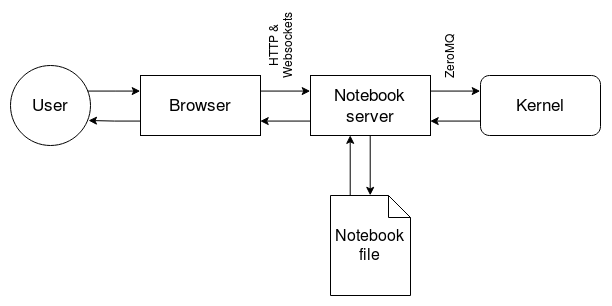
\includegraphics[width=0.8\textwidth]{jupy.png}
  \caption{Componentes de \textit{Jupyter Notebook}}
  \label{fig:components}
\end{figure}

La estructura básica de Jupyter la podemos encontrar en la figura \ref{fig:components}. En ella identificamos los tres elementos principales que componen la plataforma: El servidor de \textit{notebooks "Notebook server"}, el archivo \textit{notebook "Notebook File"} y el \textit{Kernel}. 


\subsection{Servidor de \textit{notebooks}}
\label{subsec:estructura-servidor}

Es el servicio desplegado cuando se inicia la aplicación. En él podemos ver el directorio desde el cuál se ha lanzado el proceso y seleccionar cada uno de los archivos \textit{notebook} bien para visualizarlos y ejecutarlos o para realizar alguna otra acción como eliminarlos, renombrarlos, etc.
 También podemos ver en otra pestaña qué archivos están en ejecución, y detener su \textit{kernel} asociado.
 
Estructuralmente, el servidor de notebooks es el proceso que sirve como nexo de unión entre el usuario y el notebook final, al que accederá y modificará. Implementa todas las conexiones entre el navegador y el notebook (en este caso los \textit{handlers} para las llamadas \textit{HTTP}); así como las conexiones entre el notebook y el kernel, especificadas en la documentación de \textit{Jupyter}, más concretamente en \textit{The wire protocol} \cite{wire-protocol}, que utilizan la tecnología \textit{ZMQ} \footnote{http://zeromq.org/}.

\begin{figure}[h]
	\centering
  	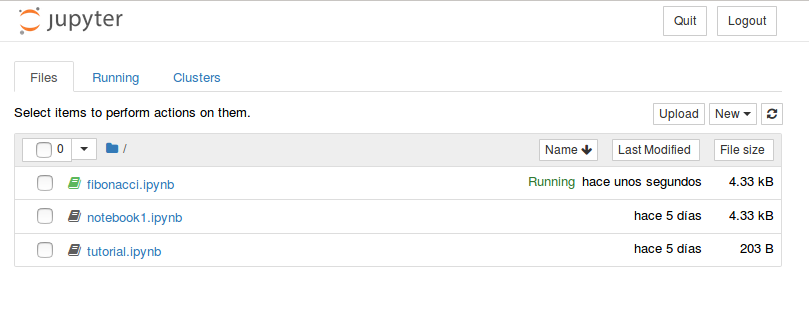
\includegraphics[width=\linewidth]{tree.png}
  	\caption{Interfaz del servidor de \textit{notebooks}}
  	\label{fig:tree}
\end{figure}

En la figura \ref{fig:tree} podemos ver una captura de la interfaz del servidor de \textit{notebooks}. Podemos identificar cada uno de los \textit{notebooks} en la lista, así como la pestaña \textit{running}, donde podríamos detener la ejecución de los \textit{kernels} en marcha.


\subsection{Archivo \textit{notebook}}
\label{subsec:estructura-notebook}

Es el documento principal dentro de todo el ecosistema de \textit{Jupyter}. Toda la plataforma va enfocada a estos archivos, donde encontramos el código y los resultados de los mismos. El notebook se divide en celdas, que son las unidades de ejecución, es decir, al ejecutar una celda, se ejecuta solamente el contenido de ésta. Las celdas se dividen en dos secciones, una para la entrada, donde el usuario introduce el código; y otra para la salida, donde, en el caso de que el código ejecutado en la casilla tenga una salida disponible, se mostrará el resultado de la ejecución. 

La función principal del \textit{notebook} es la persistencia, pues nos sirve para no perder el trabajo realizado, ya que al finalizar una sesión éste queda guardado en disco. Los notebooks tienen la extensión \textit{.ipynb}, que significa \textit{IPython notebook}. Internamente son archivos \textit{JSON}, donde encontramos una \textit{array} de celdas, con sus respectivas entradas y salidas, así como los metadatos del mismo \textit{notebook}.

La ejecución del notebook se realiza haciendo uso de los \textit{Kernels}, y la explicaré más adelante, pues hace falta tener el concepto de \textit{Kernel} claro para entender su funcionamiento.

En la figura \ref{fig:notebook} podemos ver un ejemplo de \textit{notebook}. En ella se pueden apreciar detalles, como la posibilidad de mostrar celdas formateadas en \textit{markdown} \footnote{https://es.wikipedia.org/wiki/Markdown}, o el uso de \textit{rich output}, como podemos ver en el gráfico de la parte inferior.


\subsection{\textit{Kernel}}
\label{subsec:estructura-kernel}

Es el componente encargado de la ejecución del código dentro de la plataforma \textit{Jupyter}. Se trata de un proceso externo al servidor de \textit{notebooks} donde se manda, mediante ZMQ e implementando \textit{The wire protocol} \cite{wire-protocol}, el segmento de código que se quiere ejecutar. El código será ejecutado en base al contexto (estado de las variables, funciones, etc.) que se tenga en el \textit{kernel} en ese momento, que vendrá determinado por las ejecuciones anteriores.

Existen \textit{Kernels} para más de 100 lenguajes \cite{kernel-list}, y su desarrollo es bastante sencillo, pudiéndose hacer uso de recursos como el Wrapper \footnote{http://jupyter-client.readthedocs.io/en/stable/wrapperkernels.html}, que implementa toda la mensajería que comunica el \textit{Kernel} con el cliente.

\begin{figure}[H]
	\centering
  	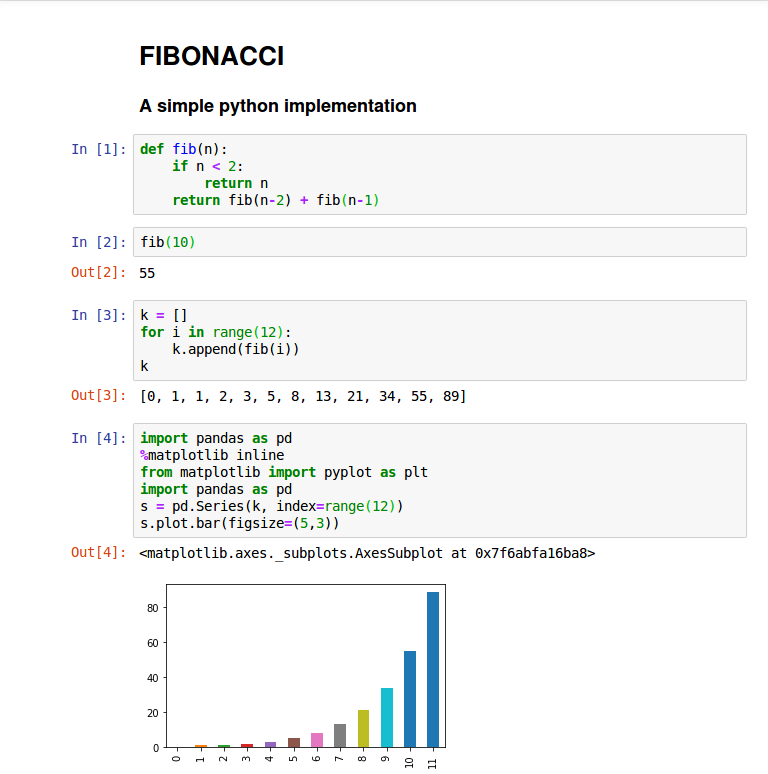
\includegraphics[width=\linewidth]{notebook.png}
  	\caption{Ejemplo de \textit{notebook}}
  	\label{fig:notebook}
\end{figure}


\subsection{Modelo de ejecución}
\label{subsec:modelo-ejec}

Una vez explicados los elementos que componen la plataforma, podemos pasar a ver su modelo de ejecución. Funciona de la siguiente manera: El código que se encuentra dentro de la casilla a ejecutar se manda al \textit{kernel}. Éste lo procesa en base a su contexto, es decir, el estado de las variables guardadas en el momento en el que se ejecuta la casilla. Ésto quiere decir que si se ejecuta una casilla con una numeración inferior más tarde que una con una numeración superior, la inferior se ejecutará en base a lo guardado por la superior. Por lo tanto, el orden de las casillas dentro del \textit{notebook} no tiene porqué corresponder con el orden en el que han sido ejecutadas, ya que el usuario es libre de ejecutar cada casilla cuando quiera. Este modelo de ejecución puede resultar confuso, y hay que tenerlo en cuenta a la hora de buscar fallos en los resultados.

Por otro lado, cuando el \textit{kernel} detecta que los restultados se pueden mostrar de más de una manera, por ejemplo, en texto plano o con un gráfico, manda todas las salidas posibles hacia el cliente, y es éste el encargado de decidir cuál le va a mostrar al usuario. Esto se debe a que los \textit{kernels} no funcionan exclusivamente con \textit{notebooks}, sino que pueden ser utilizados con otros \textit{frontends}, como podrían ser terminales o otras aproximaciones, por ejemplo \textit{qtconsole} \footnote{https://ipython.org/ipython-doc/3/interactive/qtconsole.html}.


% FORMALIZACIÓN DEL PROBLEMA

\section{Formalización del problema}
\label{sec:formalizacion}

Tal y como se comentaba en el apartado \textit{objetivos}, la finalidad del proyecto es desarrollar un entorno que permita el uso colaborativo de \textit{Jupyter}. Para ello, tenemos que cumplir objetivos más pequeños y acotados, pues todos van a desempeñar un papel necesario en el producto final. A continuación los expondré, entrando en detalles de porqué son necesarios para el proyecto.

\begin{itemize}

\item \textbf{Sincronización}. La sincronización es un aspecto fundamental para una herramienta colaborativa. Nos permite conocer el estado del documento, así como los cambios producidos por otros usuarios. 


\item \textbf{Identificación y permisos}. Es necesario diseñar un sistema para ver quién está modificando los documentos y si tiene permisos para hacerlo, así como asegurarse de que no pueda hacerlo si no los tiene. Una vez identificados los usuarios, se puede saber con quién se está colaborando.

\item \textbf{Compartición}. Hace falta una manera de poder añadir a nuevos usuarios a los documentos. No se puede  colaborar si no hay manera de que dos o más personas editen el mismo archivo.

\item \textbf{Persistencia}. Se necesita un mecanismo para mantener la identificación de los usuarios en cada una de sus sesiones. De esta manera, no será necesario que se vuelva a compartir el documento cuando un usuario salga de la aplicación y vuelva a entrar.

\end{itemize}


% ANÁLISIS DE LA SEGURIDAD

\section{Análisis de la seguridad}
\label{sec:analisis-seguridad}

Para garantizar a los usuarios que sus documentos no pueden ser vistos por personas no autorizadas, se ha de crear un modelo de seguridad en la plataforma. Éste debería estar muy relacionado con la identificación y la persistencia, pues queremos comprobar y asegurarnos de que cada usuario pertenece a solamente una persona y de que estos usuarios van a ser guardados y persistidos para conexiones futuras.

\textit{Jupyter} implementa de base un sistema de seguridad, en el que se pueden proteger los servidores de \textit{notebooks} con una contraseña. Cualquier persona que conozca esta contraseña puede entrar al servidor. Este sistema no es suficiente para nuestras especificaciones, porque no identifica al usuario. No podemos saber quién se ha conectado y, por lo tanto, no le podemos aplicar su configuración y permisos.


% IDENTIFICACIÓN Y ANÁLISIS DE SOLUCIONES POSIBLES

\section{Identificación y análisis de soluciones posibles}
\label{sec:ident-soluciones}

De la misma manera que hemos planteado y formalizado los problemas que tenemos que atacar durante la realización del proyecto, vamos a identificar y analizar las posibles soluciones para cada uno de ellos. 


\subsection{Sincronización}
\label{subsec:sincro}

Para solucionar el problema de la sincronización se planteó, en una primera instancia, una sincronización por mensajería. Para ello, se haría uso de un componente llamado \textit{Connection Bridge}, que se encargaría de las conexiones entre el \textit{kernel} y los \textit{notebooks}, interceptando tanto los mensajes provenientes del \textit{notebook} que se está modificando, para mandarlos a las otras instancias y actualizarlas; como los mensajes provenientes del \textit{kernel}, para que las salidas, o \textit{outputs}, se propaguen a todas las instancias de \textit{notebooks} conectadas. Podemos ver un esquema de su funcionamiento en la Figura \ref{fig:cb-scheme}.

\begin{figure}[h]
	\centering
  	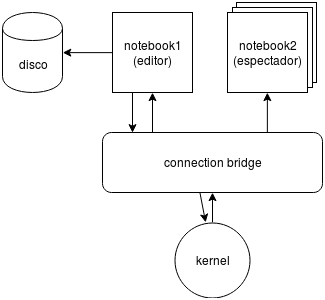
\includegraphics[width=0.5\textwidth]{Connection_Bridge.png}
  	\caption{Esquema de la sincronización con \textit{Connection Bridge}}
  	\label{fig:cb-scheme}
\end{figure}

Esta manera de sincronizar los estados de los \textit{notebooks} depende íntegramente en el funcionamiento del \textit{Connection Bridge}. Éste debe actuar como \textit{proxy}, impidiendo que el \textit{kernel} original vea que está conectado a más de un \textit{notebook}. Además tiene que implementar \textit{The wire protocol} \cite{wire-protocol} tanto en su conexion con el \textit{notebook}, pues tiene que aparecer como un \textit{kernel}; como en su conexion con el \textit{kernel}, haciéndose pasar por un cliente. 

Con este modelo, la versión del \textit{notebook} que se está modificando, es decir, la del usuario editor, será la que se persista en disco. Esa versión es la original, y no podemos asegurar que las instancias de los espectadores sean consistentes con ella. Si todos los mensajes se han mandado y recibido bien y el \textit{Connection Bridge} ha funcionado sin errores, los dos notebooks deberían ser idénticos, pero en cuanto se produzca un error no podremos estar seguros de ello.

Por otro lado, planteamos otra manera de realizar la sincronización, esta vez sin hacer uso de componentes externos. Este nuevo modelo se basa en programar que, tanto el \textit{notebook} que se está modificando como aquellos que se estén editando, se guarden o carguen con una frecuencia concreta desde disco. El hecho de realizar la sincronización de esta manera nos ofrece la ventaja de no tener que preocuparnos por las inconsistencias que podían surgir con la utilización del \textit{Connection Bridge}. Al cargar el archivo desde el disco, tenemos la certeza de que va a ser consistente. Podemos ver el esquema de este modelo en la Figura \ref{fig:disk-scheme}.

\begin{figure}[h]
	\centering
  	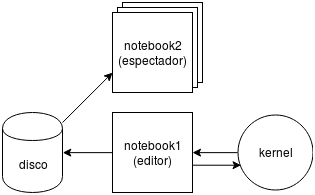
\includegraphics[width=0.5\textwidth]{JSON-sync.png}
  	\caption{Esquema de la sincronización carga desde disco}
  	\label{fig:disk-scheme}
\end{figure}


\subsection{Identificación y permisos}
\label{subsec:identificacin-permisos}

En cuanto a la identificación, se necesita un nombre público para que los usuarios se reconozcan entre sí. Internamente, cada usuario tendrá asignado un identificador único y se guardará una \textit{cookie} en el navegador durante cada sesión, para no tener que identificarlo en cada petición. No se ha planteado ninguna otra solución para el problema de la identificación.

Por otro lado, para los permisos si que se han planteado diversos modelos, desde algunos con grandes libertades para todos los usuarios y basados en la confianza hasta modelos bastante restrictivos donde la autorización para realizar las acciones está muy medida.

El modelo que más hemos estudiado es un sistema de roles, de manera que cada usuario tiene un rol en cada \textit{notebook} en el que participa. Existen cuarto roles en el sistema planteado, los cuales voy a explicar brevemente.

\begin{itemize}

\item \textbf{Administrador}: Se encarga de gestionar el \textit{notebook}, pero no lo puede modificar. Es el encargado de invitar a otros usuarios a formar parte del documento, así como de renombrarlo, o eliminarlo. También es el que controla quién modifica el \textit{notebook}, puediendo cambiar los roles del resto de usuarios. 

\item \textbf{Editor}: Es el rol que puede modificar y ejecutar los contenidos del notebook. No puede realizar ninguna función de administración.

\item \textbf{Administrador-editor}: Se trata del rol con más permisos. Es la combinación de los roles de Administrador y Editor, pudiendo llevar a cabo todas las funciones de cada uno de éstos.

\item \textbf{Espectador}: Es el rol más restrictivo. Tan solo puede acceder al documento y ver los cambios que se realizan. No pueede ni modificar ni administrar.

\end{itemize}

En la solución final elegida, sólo puede haber un administrador y un editor a la vez en cada \textit{notebook}. Por lo tanto, las dos situaciones posibles son: un Administrador-editor y \textit{N} espectadores o bien un Administrador, un Editor y \textit{N} espectadores. Los detalles de la gestión de roles se especificarán en el capítulo 4.


\subsection{Compartición}
\label{subsec:comparticion}

En lo que concierne a la compartición de documentos, se discutieron varias soluciones. Al igual que con los permisos, se puede optar por sistemas más o menos restrictivos a la hora de compartir los \textit{notebooks}, desde que todos los usuarios puedan acceder a todos los documentos hasta que tengan que ser invitados para acceder a cada uno de ellos.

Esta última opción ha sido la elegida para nuestro proyecto, pues se quiere poder mantener una privacidad dentro de la plataforma, y que solamente accedan a los documentos aquellos usuarios que han sido autorizados a ello.

Para acceder a un documento, un usuario tiene que ser invitado por un administrador, en este caso entrará como espectador al documento en cuestión; o bien puede crear un documento nuevo, en el cuál será el único usuario, y, por tanto, el Administrador-editor.


\subsection{Persistencia}
\label{subsec:persistencia}

Para la persistencia, desde el principio se planteó hacer uso de una base de datos, donde se almacenarán los usuarios, sus roles y notebooks en los que participan. Sus cararcterísticas y diseño serán mostradas en el capítulo 4, junto con más información sobre este componente.


\subsection{Seguridad}
\label{subsec:seguridad}

Por último, para la seguridad se disponía de un gran abanico de opciones, desde algunas poco robustas, como mantener la contraseña de servidor que implementa \textit{Jupyter} hasta otras como crear nuestro propio sistema de autenticación.

Se planteó hacer uso del sistema clásico de autenticación mediante usuario y contraseña, almacenando la contraseña \textit{hasheada} en la base de datos. Este modelo es suficientemente robusto para nuestro sistema, y puede ser una buena opción para solucionar el problema de la seguridad.

Por otro lado, se valoró hacer uso de una autenticación mediante terceros, haciendo uso de la tecnología \textit{OAuth} \footnote{https://oauth.net/}. Esta opción nos permite autenticar al usuario a través de otras plataformas, lo cual es una ventaja, pues no tienen que crear una cuenta explícitamente para nuestra aplicación. Estas plataformas nos facilitarán la información necesaria para identificar al usuario en nuestra aplicación.


% SOLUCIÓN PROPUESTA

\section{Solución propuesta}
\label{sec:solucion-propuesta}

En la sección anterior hemos detallado las podibles soluciones para cada uno de los problemas planteados. En este punto comentaremos cuáles han sido los elegidos para llevar a cabo en el desarrollo del proyecto.

\begin{itemize}

\item \textbf{Sincronización}: Se ha optado por el sistema de sincronización de guardado y cargado de archivos desde disco. Podemos ver su esquema en la figura \ref{fig:disk-scheme}. 

\item \textbf{Identificación y permisos}: Se ha elegido un sistema de identificación mediante un nombre de usuario público y un sistema de permisos que asigna un rol por usuario para cada notebook.

\item \textbf{Compartición}: Se utiliza un sistema de invitaciones, mediante el cuál el Administrador de un documento puede invitar a otros usuarios para que formen también parte de él.

\item \textbf{Persistencia}: Se va a hacer uso de una base de datos para almacenar la infomación que se quiere persistir.

\item \textbf{Seguridad}: Se opta por un sistema de autenticación basado en terceros, haciendo uso de la tecnología \textit{OAuth}.

\end{itemize}



%%%%%%%%%%%%%%%%%%%%%%%%%%%%%%%%%%%%%%%%%%%%%%%%%%%%%%%%%%%%%%%%%%%%%%%%%%%%%%%
%                             DISEÑO DE LA SOLUCIÓN                           %
%%%%%%%%%%%%%%%%%%%%%%%%%%%%%%%%%%%%%%%%%%%%%%%%%%%%%%%%%%%%%%%%%%%%%%%%%%%%%%%


\chapter{Diseño de la solución}
\label{ch:diseno-solu}

Tomando como punto de partida las diferentes soluciones elegidas en el capítulo anterior, se ha llevado a cabo su diseño. Este diseño de los diferentes componentes que formarán la aplicación final pasa por dos fases. La primera será un diseño general, entender el sistema como un todo y ver qué papel desempeña cada uno de los componentes dentro de éste. Trataremos este asunto en la sección \textit{Arquitectura del sistema}. Por otro lado, habrá que profundizar en cada uno de estos componentes, haciendo un estudio específico y detallado de todos ellos, aspectos que veremos en la sección \textit{Diseño detallado}. Para finalizar el capítulo, se hablará de las tecnologías utilizadas a lo largo de todo el proyecto, más concretamente en cada uno de los componentes.


% ARQUITECTURA DEL SISTEMA

\section{Arquitectura del sistema}
\label{sec:arquitectura-sistema}

\begin{figure}[h]
	\centering
  	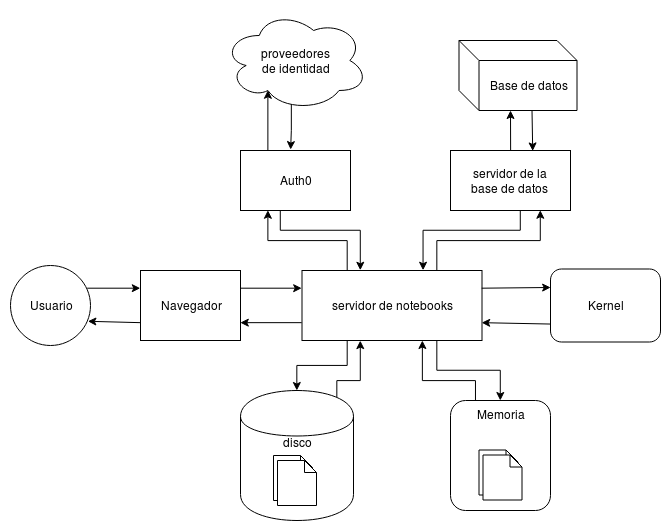
\includegraphics[width=1\textwidth]{Architecture.png}
  	\caption{Esquema general de la arquitectura del sistema}
  	\label{fig:general-arch}
\end{figure}

La arquitectura de nuestro sistema toma como base la arquitectura propia de \textit{Jupyter}, dónde la pieza principal, que sirve como nexo de unión es el servidor de \textit{notebooks}. A esta pieza se conectaban, originalmente, y como muestra la Figura \ref{fig:components}: el navegador, los \textit{notebooks} (tanto para su carga y guardado en disco como para el hecho de mantenerlos en memoria una vez estaban abiertos) y por último, los \textit{kernels}.

A parte de todos estos componentes ya nombrados, que se mantienen en el sistema final, pues se encargan de las funcionalidades indispensables de Jupyter, se van a añadir dos componentes más, que van a ser la base de datos y el sistema de autenticación. Podemos ver un esquema de la arquitectura final del sistema en la Figura \ref{fig:general-arch}.

En cuanto a las conexiones, se mantienen los protocolos utilizados originalmente, como eran \textit{HTTP} entre el navegador y el Servidor de \textit{notebooks} y \textit{ZMQ} entre entre el Servidor de \textit{notebooks} y el \textit{kernel}. 

Para los componentes nuevos, se utiliza \textit{HTTP} en ambos casos. En primer lugar, la base de datos funciona como un servicio a parte del Servidor de \textit{notebooks}. Esto quiere decir que se desplega de forma independiente, y que para acceder a los datos, el servidor de \textit{notebooks} tendrá que hacer una petición al servidor de la base de datos. Este último hará la consulta especificada y devolverá la información pertinente. Por otro lado, de la autenticación se encarga la plataforma \textit{Auth0} \footnote{https://auth0.com/}, la cual funciona como una herramienta de \textit{Authentication as a service}, y que detallaré en más profundidad en la próxima sección. La conexión entre el servidor de \textit{notebooks} y \textit{Auth0} funciona mediante redirecciones. El usuario que se tiene que autenticar es redireccionado a una \textit{URL} dentro del dominio de \textit{auth0}, y, una vez autenticado, es devuelto al servidor de \textit{notebooks}, dónde se ha enviado ya su información para poder ser identificado. 


% DISEÑO DETALLADO

\section{Diseño detallado}
\label{sec:diseno-detallado}

Una vez vista la arquitectura a nivel general que tendrá la plataforma, pasamos a ver cómo estan diseñados a nivel interno cada uno de los componentes previamente mostrados. Explicaremos  el diseño la base de datos y el sistema de autenticación, ya que, a nivel de diseño, el resto de componentes se mantienen prácticamente iguales a como lo eran en el \textit{Jupyter} original. Del funcionamiento de la herramienta resultante de nuestro proyecto hablaremos en el capítulo \ref{ch:desarrollo-solucion} \textit{Desarrollo de la solución propuesta}.


\subsection{Base de datos}
\label{subsec:diseno-bd}

Tal y como hemos explicado en el apartado anterior, la base de datos funciona como un proceso externo al servidor de \textit{notebooks}. Ésto quiere decir que para poder acceder a ella hay que lanzar el servicio. De esta manera el servidor de notebooks puede hacer peticiones al servidor de la base de datos, el cual se encargará de realizar las consultas y devolver la información que ha sido solicitada. 

Desde el punto de vista del diseño de la arquitectura, se podría haber eliminado el servidor de la base de datos, haciendo que fuera directamente el servidor de notebooks el que realizara las consultas. La ventaja de desacoplar el componente es que se puede acceder a la base de datos sin necesidad de hacerlo desde el servidor de notebooks, es decir, podemos hacer uso de la base de datos desde fuera de \textit{Jupyter}, o tener más de una aplicación haciendo peticiones simultáneamente. 

Su implementación es bastante sencilla, haciendo uso de la herramienta \textit{Tornado}  \footnote{http://www.tornadoweb.org/en/stable/} para gestionar los \textit{handlers} que se encargan de las peticiones. Por otro lado se utiliza \textit{SQLite} \footnote{https://www.sqlite.org/index.html} , que es el motor de la base de datos y la herramienta desde la cual se accede, consulta y modifica. 

En lo que respecta a la organización de la información en la base de datos, podemos ver un esquema de las tablas y columnas en la Figura \ref{fig:db-scheme}. 

\begin{figure}[h]
	\centering
  	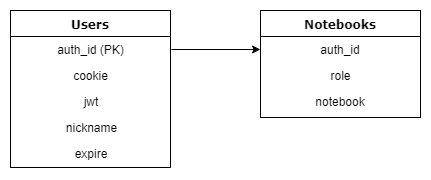
\includegraphics[width=0.75\textwidth]{database.png}
  	\caption{Esquema de tablas de la base de datos}
  	\label{fig:db-scheme}
\end{figure}

La base de datos está compuesta por dos tablas. En primer lugar la tabla \textit{Users}, donde podemos encontrar la información acerca de los usuarios registrados en la plataforma. Se compone de las siguientes columnas:

\begin{itemize}

\item \textbf{auth\_id:} Identificador único para cada usuario, es enviado por \textit{auth0} cuando el usuario se autentica. También constituye la clave primaria de la tabla.

\item \textbf{cookie:} Se guarda la cookie que genera \textit{Jupyter} para identificar la sesión del usuario. Se actualizará al cambiar de sesión.

\item \textbf{jwt:} \textit{JSON Web Token} \footnote{https://jwt.io/} , es enviado por \textit{auth0} al realizar la autenticación, y contiene información sobre el usuario. Se almacena encriptado.

\item \textbf{nickname:} Nombre de usuario que se mostrará en la plataforma. Es enviado por \textit{auth0} en base al proveedor de identidad que se escoja.

\item \textbf{expire:} Momento en el que expira el jwt generado por \textit{auth0}. El usuario se tendrá que autenticar de nuevo pasada esta fecha.

\end{itemize}

En segundo lugar, encontramos la tabla \textit{notebooks}, que muestra la información acerca de todos los archivos \textit{notebook} registrados en el servidor. Está compuesta por las colunas siguientes:

\begin{itemize}

\item \textbf{auth\_id:} Es el mismo dato que en la tabla Users. Sirve como punto para relacionar las dos tablas. 

\item \textbf{role:} Rol asignado, puede ser uno de estos cuatro valores: Administrador-editor, Administrador, Editor o Espectador.

\item \textbf{notebook:} Nombre del \textit{notebook} que se referencia. En caso de no encontrarse en el directorio \textit{root}, se mostrará la ruta para acceder a él.

\end{itemize}


\subsection{Sistema de autenticación}
\label{subsec:diseno-auth}

Para llevar a cabo el sistema de autenticación se ha hecho uso de la plataforma \textit{auth0}, como he introducido previamente en la sección Arquitectura del sistema. A continuación la introduciré y explicaré su funcionamiento.

\textit{Auth0} es una plataforma de \textit{Authentication as a Service}. Sirve para autenticar a usuarios sin necesidad de implementar nuestro propio sistema, simplemente delegando esta tarea en ella. Para conectar nuestra aplicacion con \textit{auth0} tenemos que programar una serie de redirecciones. Cuando aparece un usuario en nuestro sistema que no está identificado se le redirige a una dirección dentro del dominio de \textit{auth0}. Esta \textit{URL} está asociada a nuestra aplicación, de esta manera \textit{auth0} sabe que va a a autenticar al usuario para nuestra plataforma en concreto. Una vez aquí, el usuario tendrá diversas opciones para realizar el \textit{login}. Estas opciones se pueden seleccionar en la configuración de la aplicación en el menú de \textit{auth0}, y más adelante explicaremos cuáles hemos elegido. Una vez autenticado el usuario, se le devolverá de nuevo a nuestra aplicación, donde ya podrá funcionar con normalidad y acceder a sus documentos.

\begin{figure}[h]
	\centering
  	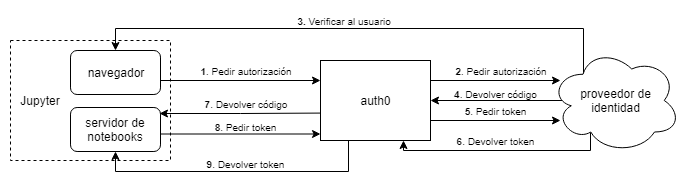
\includegraphics[width=0.9\textwidth]{auth0-flow.png}
  	\caption{Flujo de autenticación mediante \textit{auth0}, usando \textit{OAuth}}
  	\label{fig:auth0-scheme}
\end{figure}

La comunicación interna para que esto sea posible se puede ver en la Figura \ref{fig:auth0-scheme}. El proceso es el siguiente: 

El navegador se redirige a \textit{Auth0} para que el usuario se autentique (\textit{Paso 1}). \textit{Auth0} entonces solicita una autenticación al proveedor de identidad (\textit{Paso 2}). Después de verificar al usuario, pidiéndole que haga \textit{login} (\textit{Paso 3}), el proveedor de identidad le devuelve un código a a la \textit{URL} de \textit{callback} de \textit{Auth0}. Al recibir el código, \textit{Auth0} lo cambiará por un \textit{token} de acceso haciendo una petición \textit{POST} a la \textit{URL} de \textit{token} del proveedor de identidad (\textit{paso 5}) y recibirá el \textit{token} de acceso en la \textit{URL} de \textit{callback} (\textit{paso 6}). Más tarde, otra secuencia de intercambio de \textit{tokens} sucederá entre \textit{Auth0} y el servidor de \textit{notebooks}, donde \textit{Auth0} mandará un código al servidor de \textit{notebooks} (\textit{paso 7}) y el servidor cambiará el código por el \textit{token} de identificación (\textit{pasos 8 y 9}).

Este token de identificación será el que utilizemos en nuestra plataforma. Se trata de un \textit{JWT} que contiene la información sobre el usuario. Los \textit{tokens JWT} están compuestos por tres partes: Una cabezera (\textit{header}) donde aparece el algoritmo de encriptado; el contenido (\textit{payload}), de donde extraeremos la información que hemos solicitado sobre el usuario en cuestión y, por último, una firma (\textit{signature}), que se realiza utilizando la clave privada de aquél que envia el token, para verificar que proviene de donde dice provenir \footnote{https://jwt.io/introduction/}.

Una vez desencriptado el token, podemos acceder a su contenido, y recuperar aquella información que sea útil conocer para nuestra plataforma. Concretamente, nos interesa recuperar la siguiente información, que ya hemos introducido en la subsección anterior cuando hablábamos de la tabla \textit{Users} en la base de datos:

\begin{itemize}

\item \textbf{\textit{JWT}}: Guardamos el \textit{JWT}, ya que puede ser de utilidad más adelante porque contiene toda la información. Corresponderá a la columna \textit{jwt} en la base de datos.

\item \textbf{sub}: Es el identificador único del usuario. Tiene el formato (proveedor de identidad)|(id único dentro del proveedor). Un ejemplo sería \textit{github|1234567890}. Corresponderá a la columna \textit{auth\_id} en la base de datos.

\item \textbf{name}: Nombre de usuario que devuelve el proveedor de identidad. Corresponderá a la columna \textit{nickname} en la base de datos.

\item \textbf{exp}: Fecha en la que deja de ser válido el \textit{JWT}. Corresponderá a la columna \textit{expire} en la base de datos.

\end{itemize}

El diagrama de flujo que vemos en la Figura \ref{fig:auth0-scheme} corresponde a la secuencia de acciones llevadas a cabo en el caso de que el usuario se identifique con la aplicación de un tercero (el proveedor de identidad). Auth0 permite la identificación de esta manera mediante muchas plataformas, como es el caso de \textit{Google}, \textit{Github}, \textit{Linkedin}, etc \footnote{https://auth0.com/docs/connections}. Sin embargo, también ofrece la posibilidad de utilizar al propio \textit{Auth0} como proveedor de identidad. En este caso, el usuario se registra con un correo y contraseña, así como el \textit{nickname} que quiera, para ser identificado por el resto de usuarios dentro de nuestra plataforma. De esta manera, no se necesita llamar a un tercero, los pasos 2, 4, 5 y 6 vistos en el diagrama de la figura \ref{fig:auth0-scheme} se omitirían, y del paso 3 se encargaría el propio \textit{Auth0}. El esquema resultante sería el de la Figura \ref{fig:auth0-scheme-2}.  

\begin{figure}[h]
	\centering
  	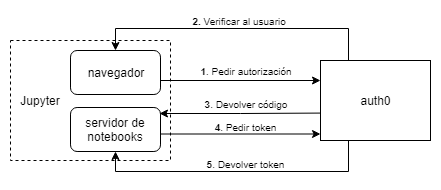
\includegraphics[width=0.75\textwidth]{auth0-flow2.png}
  	\caption{Flujo de autenticación mediante \textit{auth0} sin proveedor de identidad externo}
  	\label{fig:auth0-scheme-2}
\end{figure}

Para nuestro sistema hemos optado por ofrecer tanto la autenticación por terceros utilizando \textit{OAuth} así como la posibilidad de entrar en la plataforma mediante un correo electrónico y contraseña, que será guardado directamente en el dominio de \textit{auth0}. En la figura \ref{fig:login} podemos ver la interfaz del \textit{login} de \textit{auth0} para nuestra plataforma, donde se muestran las dos opciones previamente comentadas.

\begin{figure}[H]
	\centering
  	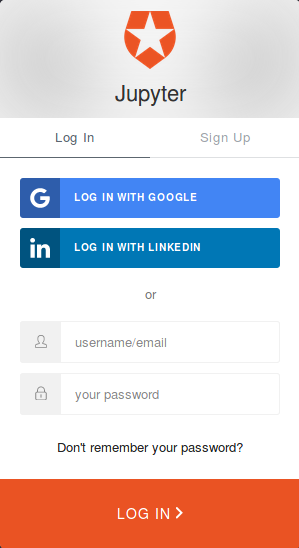
\includegraphics[width=0.5\textwidth]{login.png}
  	\caption{Interfaz de \textit{login} de \textit{auth0}}
  	\label{fig:login}
\end{figure}


% TECNOLOGÍA UTILIZADA

\section{Tecnología utilizada}
\label{sec:tecno-utilizada}

Hemos utilizado diversas herramientas y tecnologías a lo largo del desarrollo del proyecto. Hemos ido introduciendo muchas de ellas en lo que llevamos de memoria, en los puntos en los que resultaba relevante mencionarlas. Por lo tanto, esta sección servirá como un pequeño glosario donde se pueden encontrar todas las herramientas utilizadas sin entrar en grandes detalles sobre su funcionamiento. Estará estructurada por componentes, los vistos en la Figura \ref{fig:general-arch}, siendo cada uno una subsección de este punto.


\subsection{Servidor de \textit{notebooks}}
\label{subsec:tecno-server}

El servidor de notebooks utiliza una gran variedad the tecnologías. El \textit{backend} está programado en \textit{Python}, haciendo uso de \textit{Tornado} para implementar los \textit{handlers} del servicio web. En cuanto al \textit{frontend}, hace uso de \textit{JavaScript} \footnote{https://www.javascript.com/} y de \textit{HTML} \footnote{https://es.wikipedia.org/wiki/HTML}. Los archivos \textit{notebook} que encontramos en el servidor, ya sea en disco o en memoria, son documentos \textit{JSON}, así que se hace uso de esta tecnología para la persistencia de la información. Por último, las conexiones con el resto de componentes se realizan en casi todos los casos por \textit{HTTP}, siendo el kernel una excepción, pues hace uso de \textit{ZMQ}. 


\subsection{\textit{Kernels}}
\label{subsec:tecno-kernels}

Como hemos comentado anteriormente, los \textit{kernels} hacen uso de \textit{ZeroMQ} para el intercambio de información mediante mensajería, tal y como está especificado en \textit{The wire protocol} \cite{wire-protocol}. No se ha desarrollado ningún \textit{kernel} para este trabajo, pero normalmente se programan en el lenguaje que implementan. Más información en la subsección \ref{subsec:estructura-kernel}.


\subsection{Base de datos}
\label{subsec:tecno-DB}

La base de datos utiliza la herramienta \textit{SQLite} para su creación y utilización. En cuanto al servidor de la base de datos, está programado en \textit{Python}, haciendo uso de la plataforma \textit{Tornado} para los servicios \textit{web} y se comunica por \textit{HTTP} con el servidor de \textit{notebooks}.


\subsection{Sistema de autenticación}
\label{subsec:tecno-auth}

Tal y como hemos expuesto en la subsección \ref{subsec:diseno-auth}, de la autenticación se encarga la herramienta \textit{Auth0}. Ésta hace uso de tecnologías como \textit{OAuth} para identificar al usuario mediante proveedores de identidad externos. También da la posibilidad de crear una cuenta en \textit{Auth0} y que sea la propia plataforma la que autentique al usuario. Ambas opciones están contempladas en nuestra aplicación.



%%%%%%%%%%%%%%%%%%%%%%%%%%%%%%%%%%%%%%%%%%%%%%%%%%%%%%%%%%%%%%%%%%%%%%%%%%%%%%%
%                   DESARROLLO DE LA SOLUCIÓN PROPUESTA                       %
%%%%%%%%%%%%%%%%%%%%%%%%%%%%%%%%%%%%%%%%%%%%%%%%%%%%%%%%%%%%%%%%%%%%%%%%%%%%%%%


\chapter{Desarrollo de la solución propuesta}
\label{ch:desarrollo-solucion}

Una vez finalizado el diseño, se procede a la implementación de cada una de las partes o componentes especificados. Se procede de una manera escalonada durante el desarrollo del trabajo. En primer lugar se plantean los objetivos a cumplir, y tomando como base estos objetivos, se atacan uno por uno. Por lo tanto, se analiza el objetivo, se diseña su solución en concreto, se implementa y se prueba. En el momento en que el objetivo queda solucionado, se avanza al siguiente.

Se tomó como base para la implementación el repositorio de \textit{Github} de \textit{Jupyter notebook}, más concretamente su versión estable 5.5.0 \footnote{https://github.com/jupyter/notebook/releases/tag/5.5.0}. Debido al gran tamaño del repositorio, fué bastante costoso familiarizarse con él y descubrir qué archivos realizaban qué funciones. Además, hubo que aprender a utilizar las tecnologías que se empleaban en el repositorio, como por ejemplo \textit{Tornado}.

A continuación se expondrá, por orden de realización, cuál fué el proceso de desarrollo de cada uno de los objetivos.


% SINCRONIZACIÓN DE NOTEBOOKS EN TIEMPO REAL

\section{Sincronización de \textit{notebooks} en tiempo real}
\label{sec:desarrollo-sincro}

Se comenzó a realizar la implementación de la solución por este objetivo. A lo largo de todo el desarrollo y programación de las soluciones, se intentará reutilizar al máximo aquellos fragmentos de código de la plataforma original que nos puedan resultar útiles. Este es el caso de la sincronización, pues \textit{Jupyter} realiza un guardado automático en disco siguiendo un intervalo, y, al abrir un \textit{notebook} carga los contenidos desde disco.

Una vez identificados estos dos métodos, se procede a crear un intervalo en el que se llamará, según el rol del usuario en el \textit{notebook} a un método o a otro, para que la instancia que ve ese usuario sea la que se cargue o se guarde (Todavía no estaba implementado el sistema de roles pero ya estaba diseñado). Se fijó el tiempo del intervalo para la carga y guardado en dos segundos, pues es un tiempo de espera razonable, y, en caso de ser menor, el consumo de recursos se dispara, llegando a un punto insostenible.

Surgió un problema con la carga de \textit{notebooks}, porque el método que la realiza rompe el contenedor sobre el que van insertadas todas las celdas del documento, y, cuando se van a insertar las nuevas celdas que se tienen que cargar, se crea otro contenedor, forzando a la ventana a hacer un \textit{scroll} hasta arriba del todo. Ésto supone un problema para el usuario que está espectando los cambios en el \textit{notebook}, pues no puede seguir el desarrollo que se produce, ya que cada dos segundos se le cambia la vista, llevándolo a la parte superior del archivo. Se solucionó este problema mediante la modificación del método de cargado, haciendo que no se rompiera el contenedor, y que se eliminaran y cargaran las celdas una por una. De esta manera, al realizar el cargado, el usuario se mantiene en lugar en el que se encontraba previamente, haciendo que no pierda la vista en la que se encontraba.


% CREACIÓN DE UN SISTEMA DE ROLES Y PERMISOS

\section{Creación de un sistema de roles y permisos}
\label{sec:desarrollo-roles}

El desarrollo del sistema de roles va muy ligado al desarrollo de la base de datos. El sistema de roles hace muchas consultas para conocer el rol de cada usuario en cada momento, así como para realizar modificaciones en el caso de que sea necesario. 

Los roles se tienen que tener en cuenta en la aplicación principalmente en dos sitios. En primer lugar, en el ciclo de ejecución de los notebooks. Como se ha comentado en la sección \ref{sec:desarrollo-sincro} sobre la sincronización, se hace uso de un intervalo para el guardado y la carga de los archivos. En este punto se tiene que comprobar el rol de cada usuario, para saber si cargará o guardará el archivo, así como actualizar un \textit{flag} creado en la interfaz para que el usuario sepa qué rol tiene. En el caso de que el usuario tenga permisos de administración se le mostrará en un submenú sus acciones disponibles. Por otro lado, es importante conocer el rol para saber si un usuario tiene potestad para realizar ciertas acciones sobre un notebook, como por ejemplo renombrarlo o eliminarlo. En estos casos, en el propio \textit{handler} de la petición, se pedirá a la base de datos que compruebe el rol del usuario, en el caso de no tener los permisos necesarios para realizarla, se enviará el código de estado \textit{HTTP} 401, usuario no autorizado. 

El usuario encargado de la administración de un notebook puede delegar los permisos de modificación en otro usuario. Para ello, aparece el submenú \textit{Colaborator} en el menú \textit{File} en la interfaz. El submenú es un desplegable donde se muestran todos los usuarios que forman parte del notebook. Este desplegable se consigue pidiéndole la información a la base de datos, e insertando cada uno de los usuarios devueltos en el código \textit{HTML} por medio de \textit{jquery}. Cuando se hace \textit{click} en un usuario, se manda una petición a la base de datos para convertirlo en editor. Se pueden dar los siguientes casos en función del rol del usuario seleccionado:

\begin{itemize}

\item \textbf{Administrador-editor o Editor}. Todo se mantiene tal y como está, pues el usuario ya tiene premisos de edición, no hay que modificar nada.

\item \textbf{Administrador}. Si el usuario elegido es administrador quiere decir que existe un usuario con el rol de Editor. El Administrador pasa a Administrador-editor y el Editor pasa a Espectador.

\item \textbf{Espectador}. Si se trata de un espectador, se pueden dar dos casos. En primer lugar, que exista un Editor, por lo que éste pasaría a Espectador y el Espectador elegido a Editor. Por otro lado, si no existe un Editor, tiene que existir un Administrador-editor, por lo que éste pasaría a ser Administrador y el Espectador sería el nuevo Editor.

\end{itemize}

El sistema de roles no puede funcionar sin la base de datos, porque se perdería toda la información cuando el servicio se cayera y se volviera a lanzar, ya que no se podría recordar qué usuario tiene qué rol en qué notebook.


% PERSISTENCIA DE LA INFORMACIÓN NECESARIA

\section{Persistencia de la información necesaria}
\label{sec:desarrollo-persistencia}

La persistencia se llevó a cabo mediante una base de datos, cuyo diseño se ha introducido en la subsección \ref{subsec:diseno-bd}. Para su desarrollo se utilizó la herramienta \textit{SQLite}, la cuál permitió realizar una implementación sencilla y robusta. 

En un primer momento, la base de datos se accedía directamente desde el servidor de \textit{notebooks}, habiendo importado la herramienta \textit{SQLite} en este componente y realizando las llamadas en los lugares adecuados. \textit{SQLite} trabaja con código \textit{SQL} \footnote{https://es.wikipedia.org/wiki/SQL} , un lenguaje sumamente extendido,  por lo que no fué complicado programar todas las consultas necesarias para el correcto funcionamiento de la plataforma, ya que la base de datos es muy pequeña (véase la Figura \ref{fig:db-scheme}) y las consultas que se requieren son sencillas.

Más tarde, se optó por cambiar el acceso a la base de datos e implementarlo como un servicio web externo. Este cambio no supuso ningún problema a nivel de programación, y se procedió de la siguiente manera. En primer lugar se colocaron los métodos de acceso a la base de datos en un archivo python nuevo. Entonces, se metió cada método dentro de un \textit{handler} de un a petición \textit{HTTP}. Ésto se llevó a cabo haciendo uso de la plataforma \textit{Tornado}, pues ya se conocía debido a su uso en el servidor de \textit{notebooks}. Más tarde, se cambiaron los puntos donde originalmente se hacían los accesos en el servidor de notebooks por peticiones \textit{HTTP} al servidor de la base de datos. Por último, los datos que se solicitan en las peticiones se devuelven en las respuestas \textit{HTTP}, y son gestionados de forma asíncrona por el servidor de \textit{notebooks}.


% SESIONES DE LOS USUARIOS

\section{sesiones de los usuarios}
\label{sec:desarrollo-sesiones}

Mantener las sesiones de los usuarios es necesarios para que no se pierda el flujo de trabajo en el caso de que, por ejemplo, se actualice la página o se cierre el navegador. En un principio, se crearon unas \textit{cookies} que se guardaban en la base de datos e identificaban al usuario. Estas \textit{cookies} se creaban de cero, y caducaban al cabo de un tiempo, y se utilizaban para saber qué usuario estaba conectado en el navegador, manteniendo su sesión. 

Como un usuario puede conectarse a la plataforma desde otros ordenadores o navegadores, con este sistema se perdían sus datos, pues lo único que lo identificaba era la propia \textit{cookie}. Al cambiar de sistema de seguridad, y utilizar una plataforma externa como \textit{Auth0}, la cookie pasó a tener la utilidad que debe tener, es decir, mantener la sesión. Se eliminó la implementación de nuestra \textit{cookie} personalizada y pasó a utilizarse una creada por \textit{Jupyter} originalmente. Ésta se genera y guarda en la base de datos cuando un usuario se autentica. En el momento en el que el usuario se conecta desde otro navegador o ordenador, se actualiza la \textit{cookie} en la base de datos, haciendo que cualquier otra \textit{cookie} asociada a el usuario en otro navegador quede invalidada, haciendo que el usuario se tenga que volver a autenticar en ese navegador. Si la \textit{cookie} llega al punto de caducar, se exige la autenticación del usuario de nuevo.


% COMPARTICIÓN DE LOS DOCUMENTOS

\section{Compartición de los documentos}
\label{sec:desarrollo-comparticion}

Respecto a la compartición de los documentos, se ha desarrollado el siguiente sistema. Cuando un usuario entra por primera vez en la plataforma, depués de realizar el \textit{login} se encuentra con un directorio vacío, esto se debe a que no forma parte de ningún documento. El usuario tiene la opción de crear un documento, de esta manera se convertiría en el Administrador-editor de este \textit{notebook}, véase la subsección \ref{subsec:identificacin-permisos}. La otra opción de la que dispone es que el usuario con permisos de administración de otro documento le dé acceso, para ello, el Administrador deberá seleccionarlo en el submenú \textit{Add user}, en el que aparecen todos los usuarios registrados en la plataforma que no pertenezcan ya al documento.

Este submenú funciona de manera similar al explicado en la sección \ref{sec:desarrollo-roles}, insertando por medio de \textit{jquery} los diferentes usuarios dados de alta en la plataforma (tras la pertinente consulta a la base de datos) en el \textit{HTML} que se mostrará. Cuando se elige un usuario, se realiza una petición al servidor de la base de datos para generar una entrada con este usuario como Espectador en el notebook en cuestión.

A partir de este momento, se mostrará el notebook el directorio del usuario. Ésto se consigue haciendo una consulta a la base de datos para que nos devuelva la lista de notebooks en la que aparece el usuario. Esta lista, más tarde se comparará con el contenido real del directorio, y se listarán solo los \textit{notebooks} que aparecen en ambos lados.


% AUTENTICACIÓN DE LOS USUARIOS

\section{Autenticación de los usuarios}
\label{sec:desarrollo-auth}

Tal y como se ha expuesto en la sección \ref{sec:desarrollo-sesiones}, la identificación de usuarios se realizaba en primera instancia mediante la \textit{cookie} generada en el servidor de \textit{notebooks}. Al no ser éste un método lo suficientemente robusto tanto para la seguridad de la plataforma como para el uso por parte de los usuarios, se decidió cambiar.

El nuevo sistema hace uso de la plataforma \textit{Auth0} para la autenticación de los usuarios. Para poner en marcha este sistema, se creó una cuenta en \textit{Auth0} y se registró la aplicación. De esta manera, se generan unas \textit{URLs} específicas de la aplicación a las que se tiene que redirigir al usuario para que realice su \textit{login}. También son generados el identificador de la aplicación así como una clave secreta. Por último hace falta especificar la dirección a la que se debe redirigir al usuario una vez termine su autenticación, llamada \textit{callback URL}. 

Por otro lado, en el servidor de notebooks se realiza un \textit{bypass}, que consiste en redirigir a todos los usuarios no identificados en la plataforma a la \textit{URL} de \textit{login} de \textit{Auth0}. En esta \textit{URL} va incluido como argumento el identificador de nuestra aplicación. Una vez el usuario es autenticado, se devuelve al usuario a la \textit{callback URL} especificada en los ajustes de la aplicación de \textit{Auth0}. Se recibe un código, que habrá que mandar haciendo una petición tipo \textit{POST} por \textit{HTTPS} a una \textit{URL} de las generadas previamente junto con el identificador de la aplicación y la clave secreta. De esta manera, \textit{Auth0} sabe que tenemos permisos para generar los \textit{JWT}, así que se generan y se devuelven.
Podemos ver una vista detallada de esta interacción en el esquema de la Figura \ref{fig:auth0-scheme}, así como más información en la documentación de \textit{Auth0} \footnote{https://auth0.com/docs/application-auth/current/server-side-web}.

Con el \textit{JWT} correspondiente al login del usuario en nuestro dominio, se procede a desencriptarlo, haciendo uso de la clave pública de nuestra aplicación, pues viene firmado con la privada para saber que es quién dice ser. Una vez desencriptado, se guardará la información relevante en la base de datos.



%%%%%%%%%%%%%%%%%%%%%%%%%%%%%%%%%%%%%%%%%%%%%%%%%%%%%%%%%%%%%%%%%%%%%%%%%%%%%%%
%                              IMPLANTACIÓN	                                  %
%%%%%%%%%%%%%%%%%%%%%%%%%%%%%%%%%%%%%%%%%%%%%%%%%%%%%%%%%%%%%%%%%%%%%%%%%%%%%%%


\chapter{Implantación}
\label{ch:implantacion}

Para hacer uso de la aplicación y llevar a cabo su despliegue, se deben seguir una serie de pasos, ya que hay que realizar las conexiones de forma correcta, pues si no los componentes no se podrán comunicar entre ellos.

En primer lugar, hay que crear una cuenta en la plataforma \textit{Auth0} y dar de alta la aplicación. De esta manera coseguiremos el conjunto de \textit{URLs} y claves necesarias para redirigir al usuario y que se pueda autenticar. También tendremos que configurar la \textit{URL} de \textit{callback} dentro de \textit{Auth0}, para que la redirección  del usuario de vuelta a nuestra plataforma sea exitosa. Esta \textit{URL} deberá pertenecer al dominio en el que se ejecuta la aplicación, y hay que tener en cuenta que si se cambia, se tendrá que añadir la nueva dirección a \textit{Auth0}.

Una vez configurada toda la información en \textit{Auth0}, se utilizarán las \textit{URLs} y códigos generados en el servidor de \textit{notebooks}. Para ello, hay que modificar las llamadas que se hacen en la redirección del \textit{login}, introduciendo las claves y direcciones que nos proporciona \textit{Auth0}, como se ha explicado en la sección \ref{sec:desarrollo-auth}. Por otro lado, hay que ver dónde se va a lanzar el servidor de \textit{notebooks}, ya que se necesitará una dirección para que los usuarios se conecten a la plataforma.

Por último, habrá que conectar el servidor de \textit{notebooks} y la base de datos. Simplemente se tiene que especificar la dirección en la que se lanza la base de datos en el servidor de \textit{notebooks}. La base de datos no inicia ninguna comunicación, por lo que no se ha de configurar nada por su parte. 

Para poner en marcha el sistema, se ejecutarán el servidor de la base de datos y el servidor de \textit{notebooks}. El directorio que aparecerá como \textit{root} en el servidor de notebooks es aquel en el que se ejecuta la aplicación. Es necesario tener esto en cuenta, ya que si cae el servidor y se inicia desde otro punto los usuarios pueden confundirse o no saber llegar a sus archivos. \textit{Auth0} está siempre escuchando, por lo que no es necesario hacer nada explícitamente en cuanto a esta herramienta. 

%%%%%%%%%%%%%%%%%%%%%%%%%%%%%%%%%%%%%%%%%%%%%%%%%%%%%%%%%%%%%%%%%%%%%%%%%%%%%%%
%                               PRUEBAS 		                              %
%%%%%%%%%%%%%%%%%%%%%%%%%%%%%%%%%%%%%%%%%%%%%%%%%%%%%%%%%%%%%%%%%%%%%%%%%%%%%%%

\chapter{Pruebas}
\label{ch:pruebas}


%%%%%%%%%%%%%%%%%%%%%%%%%%%%%%%%%%%%%%%%%%%%%%%%%%%%%%%%%%%%%%%%%%%%%%%%%%%%%%%
%                              CONCLUSIONES                                   %
%%%%%%%%%%%%%%%%%%%%%%%%%%%%%%%%%%%%%%%%%%%%%%%%%%%%%%%%%%%%%%%%%%%%%%%%%%%%%%%


\chapter{Conclusiones}
\label{ch:conclusiones}

Para concluir la memoria, se van a recuperar los objetivos planteados en la sección \ref{sec:objetivos} de la introducción. Se analizará hasta qué punto se han cumplido esos objetivos, así como en qué aspectos se podrían mejorar. Las mejoras serán comentadas de forma breve, pues en el capítulo \ref{ch:futuro} se verán los trabajos futuros que se pueden aplicar a este proyecto. Se tratarán también los conocimientos aprendidos, así como la familiarización con nuevas tecnologías o herramientas empleadas en el desarrollo del proyecto. Por último, se finalizará el capítulo hablando de la relación del desarrollo del trabajo con los estudios cursados.


% CUMPLIMIENTO DE LOS OBJETIVOS

\section{Cumplimiento de los objetivos}
\label{sec:conc-objetivos}

\subsection{Sincronizar los \textit{notebooks} en tiempo real.}
\label{subsec:objetivos-conc-sincro}

La sincronización en tiempo real de los documentos se ha conseguido llevar a cabo. Se ha utilizado la solución que hacía uso de la carga y guardado de notebooks en disco, cuyo análisis se puede ver en la subsección \ref{subsec:sincro}. Este modelo es funcional, pero tiene muchos fallos, como pueden ser el consumo innecesario de recursos, pues se está haciendo un polling constante para cargar los archivos; así como el aumento de tiempo de interacción a medida que los \textit{notebooks} van siendo más pesados, ya que no da tiempo a que se carguen los documentos enteros dentro del intervalo especificado.

Una mejora a considerar sería, por ejemplo, la actualización únicamente de las celdas modificadas. Ésto arreglaría los dos problemas previamente comentados, pues si un documento no ha sido modificado en el intervalo de tiempo, no se cargaría nada, y, en el caso de haber modificaciones, el consumo de recursos sería pequeño independientemente del tamaño del documento. 

En conclusión, la sincronización de los \textit{notebooks} se ha conseguido, ya que hemos llegado a un punto donde se puede hacer uso de la plataforma sin que sea una gran inconveniencia. Sin embargo, hay mucho margen de mejora, y se podría llegar a soluciones más eficientes, con un menor consumo de recursos y tiempo de espera.

\subsection{Crear un sistema de roles y permisos para los usuarios.}
\label{subsec:objetivos-conc-roles}

La creación de un sistema de roles se ha realizado correctamente. Todos los permisos que se pretenden representar en la aplicación están incluídos en algún rol. Los roles están bien diferenciados y cumplen su función dentro del entorno colaborativo. 

El sistema que se ha implementado en el proyecto solo permite un editor a la vez. La colaboración se consigue pasando el rol de editor entre los diferentes usuarios, así como haciendo que todos ellos vean los cambios en tiempo real. Una de las mejoras que podría tener nuestro sistema sería la posibilidad que se editara simultáneamente el documento por más de un usuario. Ésto es un tema delicado, pues el diseño de un sistema con más de un editor concurrente presente diversas complicaciones. Esta idea se detallará en el capítulo \ref{ch:futuro}.

Por tanto, la creación del sistema de roles se puede considerar exitosa. En cuanto al modelo de interacción, el elegido es posible que resulte un poco simple y limitado, y sería un aspecto a mejorar en veriones futuras, aunque cumple su trabajo y permite una colaboración fluida. 

\subsection{Autenticar a los usuarios.}
\label{subsec:objetivos-conc-auth}

El objetivo de la autenticación se ha cumplido con creces. La plataforma \textit{Auth0} nos ofrece una autenticación segura y robusta, haciendo uso de tecnologías muy extendidas como \textit{OAuth}. Es una solución sencilla para los usuarios, ya que pueden utilizar la identificación de un tercero o bien crear una cuenta con su usuario y contaseña. 

\textit{Auth0} nos permite añadir más capas de seguridad, como aumentar los requisitos necesarios para las contraseñas en nuestro sistema o utilizar verificación en dos pasos. No se ha hecho uso de estas opciones en la aplicación porque no se estiman necesarias, sin embargo, en caso de querer utilizarse, es tan sencillo como seleccionarlo en el menú de configuración de \textit{Auth0}, por lo que sería un cambio immediato.

En conclusión, la autenticación se ha realizado de una manera muy completa, utilizando tecnología sencilla, moderna y robusta.

\subsection{Compartir los documentos.}
\label{subsec:objetivos-conc-compartir}

Es posible compartir los documentos dentro de la plataforma, pero es un aspecto que esta sujeto a mejoras considerables. El sistema de compartición actual muestra una lista de usuarios registrados en la plataforma. De esta manera se puede seleccionar al usuario que se quiere invitar al documento para que pase a formar parte de él. Uno de los problemas que plantea este sistema es precisamente el hecho de que los usuarios que se quieren añadir a un documento tienen que estar obligatoriamente dados de alta en la plataforma.

Una solución para este problema sería dispoer de la posibilidad de compartir el documento bien mediante un link o un correo electrónico, de esta manera se podría invitar a usuarios externos a la plataforma a participar en documentos, haciendo que se registraran a través del enlace recibido y aparecieran directamente como Espectadores en el documento en cuestión.

Por lo tanto, la compartición de los documentos es posible y funcional, aunque se podría mejorar para aumentar su versatilidad.

\subsection{Persistir la información necesaria.}
\label{subsec:objetivos-conc-persistir}

La persistencia de la información se ha conseguido mediante el uso de una base de datos. Cumple todas las funciones que se requieren para el componente, por lo que el objetivo queda bastante completo.En cuanto a las mejoras disponibles, por el momento no es necesario almacenar más información. En el caso de hacer falta, se debería rediseñar la estructura de tablas de la base de datos en función a la necesidad. 

En conclusión, la base de datos es una solución completa para el problema de la persistencia, y se puede modificar para adaptarse a la información necesaria en caso de ésta cambiara.

\subsection{Mantener las sesiones de los usuarios.}
\label{subsec:objetivos-conc-session}

El guardado de las sesiones de los usuarios se ha conseguido haciendo uso de \textit{cookies}. Se utiliza una \textit{cookie} que genera el servidor de notebooks, y que funciona como identificador del usuario. Esta \textit{cookie} se almacena en la base de datos y obliga a que el usuario se vuelva a autenticar una vez caduca.

Se trata de una solución muy común para mantener las sesiones, y que, en el caso de nuestra aplicación, funciona correctamente. Por lo tanto, podemos decir que el objetivo está cumplido.


% CONOCIMIENTOS ADQUIRIDOS

\section{Conocimientos adquiridos}
\label{sec:conocimientos-adquiridos}

A lo largo del desarrollo del proyecto he trabajado con tecnologías que no había tratado durante los cuatro años del grado. Ésto me ha hecho tener que investigarlas, leer sobre ellas, buscar ejemplos e intentar conocer su funcionamiento para poder utilizarlas en la aplicación que se desarrollaba. He seguido un procedimiento bastante autodidacta, aprendiendo por mí mismo a enfrentarme a un problema, buscar soluciones, compararlas y elegir aquella que mejor se adapte al problema planteado.

Por otro lado, he aprendido a trabajar en un entorno real y con una aplicación establecida y profesional. El hecho de tomar como punto de partida para el proyecto el repositorio de \textit{Jupyter} me ha ayudado a comprender la forma de trabajar de un equipo de expertos, me ha acercado al mundo del software libre y me ha obligado a estructurar mejor mi código, siguiendo las guias de estilo de la plataforma.

A continuación, mostraré una breve lista de aspectos concretos y tecnologías que he utilizado y aprendido a lo largo del proyecto:

\begin{itemize}

\item Funcionamiento del protocolo \textit{HTTP}, así como la creación de un servidor web y el uso de la herramienta \textit{Tornado}

\item Conocimiento de la plataforma \textit{Auth0}, su uso e integración en una aplicación, además del protocolo \textit{OAuth}.

\item Ampliación de mis conocimientos sobre bases de datos, así como la puesta en marcha y uso de una.

\item Trabajo con navegadores, \textit{HTML} y \textit{JavaScript} en ellos, además del uso y programación de \textit{cookies} 
\end{itemize}

Pienso que este trabajo ha sido muy beneficioso para mí, pues he aprendido mucho de él. Todos estos aspectos mencionados anteriormente no los aprendí en el grado, pero si que he puesto en práctica muchas otras cosas aprendidas en ese periodo, como comentaré en la sección \ref{sec:estudios-cursados}.

% RELACIÓN DEL TRABAJO DESARROLLADO CON LOS ESTUDIOS CURSADOS

\section{Relación del trabajo desarrollado con los estudios cursados}
\label{sec:estudios-cursados}

Los conocimientos que adquirí en el grado en igeniería informática han tenido una gran importancia en el desarrollo de este proyecto. Desde mi punto de vista, la carrera me ha formado a un nivel básico en la gran mayoría de áreas de la informática, y ha profundizado en algunas de ellas, más concretamente en los campos relacionados con la rama que yo elegí, la computación. Han sido los primeros los que más han intervenido en el desarrollo de este proyecto.

Haciendo un barrido de términos generales a específicos, los contenidos aprendidos en el grado aplicados en este trabajo, han sido los siguientes: 

\begin{itemize}

\item \textbf{Programación}: Este proyecto habría sido imposible de llevar a cabo sin los conocimientos sobre programación aprendidos. La programación es un concepto muy amplio, y se ha tratado desde muchos puntos de vista en los estudios cursados, así que es complicado definir bien todos y cada uno de los aspectos que se han utilizado. Algunos ejemplos son el uso de clases y objetos, la herencia o las estructuras de datos. En cuanto a lenguajes de programación, había trabajado ya con algunos de los utilizados, como son \textit{Python} y \textit{JavaScript}.

\item \textbf{Bases de datos}: En el transcurso de la carrera, se había trabajado con bases de datos, lo que ha hecho que la implementación de este aspecto en concreto haya sido extremadamente sencilla. Ya conocía el lenguaje \textit{SQL}, así que he podido realizar las consultas sin que eso supusiera un gran esfuerzo. Es cierto que nunca había creado y puesto en marcha una base de datos desde cero, por lo que he ampliado mi conocimiento en ese punto.

\item \textbf{Diseño de \textit{software}}: Los conocimientos aprendidos sobre el desarrollo de \textit{software} han sido de gran importancia al diseñar la arquitectura del sistema, los componentes y sus interacciones. Es de primordial esquematizar y planificar cómo se va a afrontar el problema antes de empezar a implementar la solución.

\item \textbf{Redes y mensajería}: Ha sido de gran ayuda el conocimiento sobre redes aprendido en el grado, pues se ha hecho uso de protocolos como el \textit{HTTP}. Aunque no se había trabajado con este protocolo en mucho detalle, los conocimientos de la materia me han hecho mas llevadero el proceso. En cuanto a la mensajería, he utilizado lo aprendido para comprender el funcionamiento de los mensajes entre el servidor y los kernels. De hecho, ya había trabajado específicamente con la herramienta \textit{ZeroMQ}.

\end{itemize}

A parte de los aspectos técnicos aprendidos, cabe destacar la importancia que tiene el hecho de trabajar la resolución de problemas. En el transcurso del grado, se insiste en que el alumnado se enfrente a problemas de manera independiente. De esta manera , cuando el alumno se enfrenta a un problema real, sabe por donde atacarlo y puede llegar a conclusiones y resultados por si mismo. Estos conocimientos han sido vitales a la hora de realizar el trabajo, pues se trata de un desarrollo en solitario, y puede resultar abrumador plantear problemas sin tener un conocimiento básico de como empezar a resolverlos.

%%%%%%%%%%%%%%%%%%%%%%%%%%%%%%%%%%%%%%%%%%%%%%%%%%%%%%%%%%%%%%%%%%%%%%%%%%%%%%%
%                          TRABAJOS FUTUROS                                   %
%%%%%%%%%%%%%%%%%%%%%%%%%%%%%%%%%%%%%%%%%%%%%%%%%%%%%%%%%%%%%%%%%%%%%%%%%%%%%%%



\chapter{Trabajos futuros}
\label{ch:futuro}


Tal y como se ha comentado en el capítulo \ref{ch:conclusiones}, existe un gran margen de mejora para nuestra aplicación. El objetivo principal, que era la creación de un entorno colaborativo se ha logrado, sin embargo, éste podría ser más completo. Se debe tener en cuenta que el Trabajo de Fin de Grado tiene una carga lectiva determinada, en concreto 12 créditos \textit{ECTS}, así como unos plazos establecidos, por lo que en elgún momento se tiene que detener el desarrollo del proyecto. Éste ha sido el motivo principal por el que estos trabajos futuros que se expondrán a continuación no han podido ser incorporados en el proyecto realizado.

Los dos aspectos que disponen de un margen de mejora más amplio, desde mi punto de vista, son la sincronización de los \textit{notebooks} y el modelo de edición y ejecución de nuestra plataforma, como se comenta en las subsecciones \ref{subsec:objetivos-conc-sincro} y \ref{subsec:objetivos-conc-roles} respectivamente. Se han planteado y diseñado algunas mejoras para estos dos objetivos del proyecto, como vamos a ver en las secciones de este capítulo.


%MEJORAS EN LA SINCRONIZACIÓN DE NOTEBOOKS

\section{Mejoras en la sincronización de \textit{notebooks}}
\label{sec:mejoras-sincro}

Se ha tratado en diferentes apartados de la memoria, como en la subsección \ref{subsec:sincro} o en la sección \ref{sec:desarrollo-sincro}, la solución llevada a cabo en el proyecto frente al problema de la sincronización. Consiste en sincronizar los diferentes documentos mediante la carga y guardado en disco de éstos. 
Esta solución se puede mejorar, tanto en el aspecto de la eficiencia, consumiendo menos recursos, así como en velocidad, reduciendo el tiempo de espera que existe entre que una modificación es realizada hasta que es vista por los espectadores.

La mejora propuesta consiste en realizar la carga de los documentos celda por celda. En el sistema actual, se carga el documento entero cada vez, lo que quiere decir que independientemente de los cambios que se hagan, se va a tardar lo mismo, pues se realiza una carga del archivo al completo. Con el nuevo sistema, el tiempo de carga dependerá del tamaño de las modificaciones realizadas desde el último guardado. Como el intervalo de tiempo utilizado es tan solo dos degundos, se puede esperar que estos cambios sean pequeños generalmente. Además, como solamente se actualizan las celdas modificadas, en el caso de no haberse producido ningún cambio desde el último guardado, el \textit{notebook} directamente no se actualizará, por lo que se ahorrará en recursos en aquellos  ciclos en los que el \textit{notebook} no contemple cambios.

Para llevar a cabo esta mejora, se debe implementar un método de detectar qué celdas han sido alteradas y qué casillas permanecen iguales. Uno de los problemas que puede surgir es que las celdas no tienen una numeración explícita dentro del \textit{JSON}, simplemente se ordenan por orden de aparición. \textit{Jupyter} nos da la opción de cambiar el orden de las celdas o incluso de fusionar dos celdas en una. Ésto puede ser una fuente de problemas a la hora de realizar las actualizaciones celda por celda. Se puede detectar de manera sencilla qué celdas han sido modificadas, pero al no tener una numeración explícita, no se pueden relacionar en el caso de haber cambiado de orden. Por ejemplo, si se intercambia el orden de las celdas 1 y 2, acción que \textit{Jupyter} permite, nuestro sistema actualizaría las dos celdas en el documento del espectador, en lugar de intercambiarlas, ya que detectaría que las dos han sido modificadas. Este caso no es problemático, porque se puede asumir el coste de actualizar dos celdas. Sin embargo, si se fusionan las dos primeras celdas de un documento, el sistema relacionaría la celda 1 del nuevo documento (originalmente celdas 1 y 2) con la celda 1 del antiguo, la celda 2 del nuevo (originalmente la 3) con la 2 del antiguo, etc. Ésto resultaría en una actualización total del documento, ya que, desde el punto de vista del sistema, se han cambiado todas las celdas. 

La solución a este problema es mantener las relaciones de igualdad entre celdas independientemente del lugar que ocupen en el documento, es decir, saber detectar si la antigua celda 4 es la nueva 5, analizando si algunas celdas han sido añadidas o eliminadas. Siguiendo este modelo, a la hora de cargar el nuevo notebook, para cada celda del antiguo se podrán realizar cuatro acciones:

\begin{itemize}

\item \textbf{Crear la celda}. En el caso en el que se detecte que una celda ha sido añadida en algún punto, moviendo todas las celdas posteriores, se tendrá que crear una nueva celda en el notebook espectador.

\item \textbf{Actualizar la celda}. Consiste en el borrado y cargado de la celda en cuestión, se dará en el caso de que la celda haya sido modificada, pues no afecta a la alineación del resto de celdas.

\item \textbf{Eliminar la celda}. Si una celda ha sido borrada por el editor, se deberá eliminar consecuentemente en el notebook del espectador.

\item \textbf{No alterar la celda}. En el caso de que la celda mantenga su posición y contenido, no hay realizar ninguna acción.

\end{itemize}

Para saber qué celdas se tienen que crear, actualizar o modificar, el proceso encargado de la comparación tiene que identificarlas y mandarlas para que el Espectador pueda actuar en consecuencia. 

\begin{figure}[H]
	\centering
  	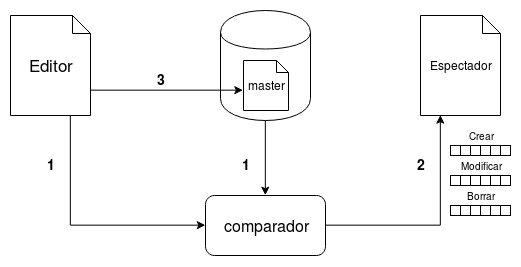
\includegraphics[width=0.9\textwidth]{nueva-sincro.png}
  	\caption{Esquema del ciclo de ejecución de la nueva sincronización}
  	\label{fig:new-sync}
\end{figure}

El ciclo de ejecución de este nuevo modelo se puede apreciar en la Figura \ref{fig:new-sync}. Podemos ver como se envian los dos documentos al proceso de comparación, el \textit{notebook} del editor, que contiene los cambios realizados desde el último guardado, y el \textit{notebook master}, que es el notebook guardado en el ciclo anterior (\textit{paso 1}). El proceso encargado de comparar los dos notebooks (comparador) estudiará los cambios realizados en el \textit{notebook} Editor respecto al \textit{master} y los agrupará en casillas creadas, modificadas y eliminadas. creará tres \textit{arrays} con los índices de las casillas en cada caso y los enviará al Espectador (\textit{paso 2}). El espectador se encargará de actualizar su versión del \textit{notebook} en base a las \textit{arrays} recibidas. Por último, se guardará el \textit{notebook} Editor en disco, para ser tratado como \textit{master} en la próxima iteración (\textit{paso 3}).


% MEJORAS EN LA EDICIÓN Y EJECUCIÓN DE LA PLATAFORMA

\section{Mejoras en la edición y ejecución de la plataforma}
\label{sec:mejoras-ejec}

El modelo de edición y ejecución de nuestra aplicación ha sido comentado en la subsección \ref{subsec:identificacin-permisos} y la sección \ref{sec:desarrollo-roles}. Se trata de un modelo con tan solo un editor concurrente, en el que ese permiso se va pasando por los diferentes usuarios con acceso al notebook que se está editando para conseguir la colaboración. El modelo de ejecución se mantenía inalterado con respecto al \textit{Jupyter} original, pues al tener solamente un editor en cada momento, todas las ejecuciones de celdas van a ser secuenciales, es decir, independientemente del usuario que esté editando, en ese momento solo ese usuario podrá ejecutar las celdas del notebook.

El modelo de ejecución de \textit{Jupyter} funciona de una forma peculiar, como se explicó en la subsección \ref{subsec:modelo-ejec}. Las casillas se ejecutan en base al contexto guardado en el \textit{Kernel} en el momento en el que se envian. Este contexto del \textit{Kernel} está formado por el estado asignado a las variables en las ejecuciones anteriores. 

Al solo poder ser editados los documentos por un usuario en el \textit{Jupyter} original, este modelo tiene sentido, porque es el usuario el que decide en que orden ejecuta las casillas, y, por tanto, el  responsable de llevar el control de el contexto en cada punto. En el momento en el que se pretende que más de un usuario pueda realizar ejecuciones en un mismo documento, el modelo de ejecución original de Jupyter empieza a no cumplir su funcióm de una forma efectiva, pues las ejecuciones de un usuario pueden romper el contexto que otro esperaba en cierto punto del \textit{notebook}.

Imaginemos que el usuario \textit{A} está editando la casilla 3 del documento, y, a su vez, el usuario \textit{B} está modificando la casilla 5. El usuario \textit{B} había preparado una variable llamada \textit{sol} en la casilla 4, para su uso posterior. Si el usuario \textit{A} utiliza esa estiqueta para cualquier otra variable y ejecuta, cuando \textit{B} intente ejecutar la casilla 5, su resultado no será el esperado, pues el valor de esa variable habrá cambiado en el contexto del \textit{Kernel}, y se aplicará el último valor guardado, devolviendo un resultado diferente al esperado por \textit{B}.

Esta situación es dificil de resolver, porque se necesita que cada usuario pueda realizar las ejecuciones dentro del contexto que necesite, y, a su vez, que los espectadores puedan ver el progreso del notebook. Si se continua funcionando como hasta ahora, se podría hacer que cada usuario tuviera una instancia del notebook diferente, y asignar un \textit{kernel} a cada uno de ellos. De esta manera, cada usuario contaría con su contexto independiente, pero ¿cómo se mustra la información en tiempo real a los espectadores? ¿Y cómo se resuelven los conflictos que se puedan generar?, por ejemplo en el caso de que diferentes usuarios hayan modificado la misma celda. Estas preguntas no tienen una respuesta sencilla, por lo que se plantea la colaboración de dos o más usuarios simultáneos haciendo uso de un modelo diferente, en el cuál a cada usuario se le deja modificar únicamente una casilla en cada momento.




%%%%%%%%%%%%%%%%%%%%%%%%%%%%%%%%%%%%%%%%%%%%%%%%%%%%%%%%%%%%%%%%%%%%%%%%%%%%%%%
%                                GLOSARIO                                     %
%%%%%%%%%%%%%%%%%%%%%%%%%%%%%%%%%%%%%%%%%%%%%%%%%%%%%%%%%%%%%%%%%%%%%%%%%%%%%%%


\printglossary[title=Glosario]



%%%%%%%%%%%%%%%%%%%%%%%%%%%%%%%%%%%%%%%%%%%%%%%%%%%%%%%%%%%%%%%%%%%%%%%%%%%%%%%
%                                BIBLIOGRAFIA                                 %
%%%%%%%%%%%%%%%%%%%%%%%%%%%%%%%%%%%%%%%%%%%%%%%%%%%%%%%%%%%%%%%%%%%%%%%%%%%%%%%


\begin{thebibliography}{10}
%%%%%%%%%%%%%%%%%%%%%%%%%%%%%%%%%%%%%%%%%%%%%%%%%%%%%%%%%%%%%%%%%%%%%%%%%%%%%%%
% MODEL D'ARTICLE                                                             %
%%%%%%%%%%%%%%%%%%%%%%%%%%%%%%%%%%%%%%%%%%%%%%%%%%%%%%%%%%%%%%%%%%%%%%%%%%%%%%%
\bibitem{light}
   Jennifer~S. Light.
   \newblock When computers were women.
   \newblock \textit{Technology and Culture}, 40:3:455--483, juliol, 1999.

%%%%%%%%%%%%%%%%%%%%%%%%%%%%%%%%%%%%%%%%%%%%%%%%%%%%%%%%%%%%%%%%%%%%%%%%%%%%%%%
% MODEL DE LLIBRE                                                             %
%%%%%%%%%%%%%%%%%%%%%%%%%%%%%%%%%%%%%%%%%%%%%%%%%%%%%%%%%%%%%%%%%%%%%%%%%%%%%%%
\bibitem{ifrah}
   Georges Ifrah.
   \newblock \textit{Historia universal de las cifras}.
   \newblock Espasa Calpe, S.A., Madrid, sisena edició, 2008.

%%%%%%%%%%%%%%%%%%%%%%%%%%%%%%%%%%%%%%%%%%%%%%%%%%%%%%%%%%%%%%%%%%%%%%%%%%%%%%%
% MODEL D'URL                                                                 %
%%%%%%%%%%%%%%%%%%%%%%%%%%%%%%%%%%%%%%%%%%%%%%%%%%%%%%%%%%%%%%%%%%%%%%%%%%%%%%%
\bibitem{WAR}
   Comunicat de premsa del Departament de la Guerra, 
   emés el 16 de febrer de 1946. 
   \newblock Consultat a 
   \url{http://americanhistory.si.edu/comphist/pr1.pdf}.

\bibitem{wire-protocol}
	\textit{The wire protocol}, el protocolo de mensajería 
    cliente-\textit{kernel} de \textit{Jupyter}.
    \newblock Consultado el 19/06/2018 en
	\url{http://jupyter-client.readthedocs.io/en/stable/messaging.html}

\bibitem{kernel-list}
	Lista de \textit{kernels} para \textit{Jupyter}.
    \newblock Consultado el 19/06/2018 en
	\url{https://github.com/jupyter/jupyter/wiki/Jupyter-kernels}

\bibitem{kernel-wrapper}
	\textit{Wrapper} para el desarrollo de \textit{kernels} para \textit{Jupyter}.
    \newblock Consultado el 19/06/2018 en
	\url{http://jupyter-client.readthedocs.io/en/stable/wrapperkernels.html}

\end{thebibliography}
\cleardoublepage

%%%%%%%%%%%%%%%%%%%%%%%%%%%%%%%%%%%%%%%%%%%%%%%%%%%%%%%%%%%%%%%%%%%%%%%%%%%%%%%
%                           APÈNDIXS  (Si n'hi ha!)                           %
%%%%%%%%%%%%%%%%%%%%%%%%%%%%%%%%%%%%%%%%%%%%%%%%%%%%%%%%%%%%%%%%%%%%%%%%%%%%%%%

\APPENDIX

%%%%%%%%%%%%%%%%%%%%%%%%%%%%%%%%%%%%%%%%%%%%%%%%%%%%%%%%%%%%%%%%%%%%%%%%%%%%%%%
%                         LA CONFIGURACIO DEL SISTEMA                         %
%%%%%%%%%%%%%%%%%%%%%%%%%%%%%%%%%%%%%%%%%%%%%%%%%%%%%%%%%%%%%%%%%%%%%%%%%%%%%%%

\chapter{Configuració del sistema}

????? ????????????? ????????????? ????????????? ????????????? ?????????????

\section{Fase d'inicialització}

????? ????????????? ????????????? ????????????? ????????????? ?????????????

\section{Identificació de dispositius}

????? ????????????? ????????????? ????????????? ????????????? ?????????????

%%%%%%%%%%%%%%%%%%%%%%%%%%%%%%%%%%%%%%%%%%%%%%%%%%%%%%%%%%%%%%%%%%%%%%%%%%%%%%%
%                               ALTRES  APÈNDIXS                              %
%%%%%%%%%%%%%%%%%%%%%%%%%%%%%%%%%%%%%%%%%%%%%%%%%%%%%%%%%%%%%%%%%%%%%%%%%%%%%%%


\chapter{??? ???????????? ????}

????? ????????????? ????????????? ????????????? ????????????? ????????????? 



%%%%%%%%%%%%%%%%%%%%%%%%%%%%%%%%%%%%%%%%%%%%%%%%%%%%%%%%%%%%%%%%%%%%%%%%%%%%%%%
%                              FI DEL DOCUMENT                                %
%%%%%%%%%%%%%%%%%%%%%%%%%%%%%%%%%%%%%%%%%%%%%%%%%%%%%%%%%%%%%%%%%%%%%%%%%%%%%%%

\end{document}
